%%%%%%%%%%%%%%%%%%%%%%%%%%%%%%%%%%%%%%%%%
% Programming/Coding Assignment
% LaTeX Template
%
% This template has been downloaded from:
% http://www.latextemplates.com
%
% Original author:
% Ted Pavlic (http://www.tedpavlic.com)
%
% Note:
% The \lipsum[#] commands throughout this template generate dummy text
% to fill the template out. These commands should all be removed when 
% writing assignment content.
%
% This template uses a Perl script as an example snippet of code, most other
% languages are also usable. Configure them in the "CODE INCLUSION 
% CONFIGURATION" section.
%
%%%%%%%%%%%%%%%%%%%%%%%%%%%%%%%%%%%%%%%%%

%----------------------------------------------------------------------------------------
%	PACKAGES AND OTHER DOCUMENT CONFIGURATIONS
%----------------------------------------------------------------------------------------

\documentclass{article}

\usepackage{fancyhdr} % Required for custom headers
\usepackage{lastpage} % Required to determine the last page for the footer
\usepackage{extramarks} % Required for headers and footers
\usepackage[usenames,dvipsnames]{color} % Required for custom colors
\usepackage{graphicx} % Required to insert images
\usepackage{listings} % Required for insertion of code
\usepackage{courier} % Required for the courier font
\usepackage{multirow}
\usepackage{hyperref}


% Margins
\topmargin=-0.45in
\evensidemargin=0in
\oddsidemargin=0in
\textwidth=6.5in
\textheight=9.0in
\headsep=0.25in

\linespread{1.1} % Line spacing

%----------------------------------------------------------------------------------------
%	CODE INCLUSION CONFIGURATION
%----------------------------------------------------------------------------------------

\definecolor{MyDarkGreen}{rgb}{0.0,0.4,0.0} % This is the color used for comments
\lstloadlanguages{c} % Load Perl syntax for listings, for a list of other languages supported see: ftp://ftp.tex.ac.uk/tex-archive/macros/latex/contrib/listings/listings.pdf
\lstset{language=[sharp]c, % Use Perl in this example
        frame=single, % Single frame around code
        basicstyle=\small\ttfamily, % Use small true type font
        keywordstyle=[1]\color{Blue}\bf, % Perl functions bold and blue
        keywordstyle=[2]\color{Purple}, % Perl function arguments purple
        keywordstyle=[3]\color{Blue}\underbar, % Custom functions underlined and blue
        identifierstyle=, % Nothing special about identifiers                                         
        commentstyle=\usefont{T1}{pcr}{m}{sl}\color{MyDarkGreen}\small, % Comments small dark green courier font
        stringstyle=\color{Purple}, % Strings are purple
        showstringspaces=false, % Don't put marks in string spaces
        tabsize=5, % 5 spaces per tab
        %
        % Put standard Perl functions not included in the default language here
        morekeywords={rand},
        %
        % Put Perl function parameters here
        morekeywords=[2]{on, off, interp},
        %
        % Put user defined functions here
        morekeywords=[3]{test},
       	%
        morecomment=[l][\color{Blue}]{...}, % Line continuation (...) like blue comment
        numbers=left, % Line numbers on left
        firstnumber=1, % Line numbers start with line 1
        numberstyle=\tiny\color{Blue}, % Line numbers are blue and small
        stepnumber=5 % Line numbers go in steps of 5
}

\newcommand{\horrule}[1]{\rule{\linewidth}{#1}}

% Creates a new command to include a perl script, the first parameter is the filename of the script (without .pl), the second parameter is the caption
\newcommand{\perlscript}[2]{
\begin{itemize}
\item[]\lstinputlisting[caption=#2,label=#1]{#1.cs}
\end{itemize}
}

\begin{document}

\begin{tabular}{l l}
\multirow{5}{*}{\includegraphics[width=2cm]{../../Recursos/logo.png}} & Universidad del Istmo de Guatemala \\
 & Facultad de Ingenieria \\
 & Ing. en Sistemas \\
 & Informatica 2 \\
 & Prof. Ernesto Rodriguez - \href{mailto:erodriguez@unis.edu.gt}{erodriguez@unis.edu.gt} \\
\end{tabular}
\\\\\\

\begin{center}
        \horrule{0.5pt}
        \huge{Hoja de trabajo \#5} \\
        \large{Fecha de entrega: 12 de Abril, 2018 - 11:59pm} \\
        \horrule{1pt}
\end{center}
\emph{Instrucciones: Realizar cada uno de los ejercicios siguiendo sus respectivas
instrucciones. El trabajo debe ser entregado a traves de Github, en su repositorio del curso, colocado en una carpeta llamada ``Hoja de trabajo 7''.
Al menos que la pregunta indique diferente, todas las respuestas a preguntas escritas deben presentarse en
un documento formato pdf, el cual haya sido generado mediante Latex. Los ejercicios de programaci\'on deben ser colocados en una carpeta
llamada ``Programas", la cual debe colocarse dentro de la carpeta correspondiente a esta hoja de trabajo.}

\section*{Iniciaci\'on}

Crear una soluci\'on llamada \emph{BinaryTree}. Dentro de esta soluci\'on crear:
\begin{itemize}
        \item{un proyecto llamado \emph{BinaryTree} de tipo console}
        \item{un proyecto llamado \emph{BinaryTreeTests} de tipo xunit}
\end{itemize}

\section*{Arbol binario mutable (10\%)}
Agregar la clase e interfaz \emph{IBinTree} y \emph{BinaryTree} que se encuentra en los ejemplos
de esta carpeta ``Semana 10'' al proyecto \emph{BinaryTree}.

Modificar la interfaz \emph{IBinTree} (y la clase \emph{BinaryTree}) de tal forma que su sus propiedades \emph{Derecho}, \emph{Izquierdo} y \emph{Valor} sean
modificables utilizando la palabra reservada \texttt{set}.
% \perlscript{homework_example}{Sample Perl Script With Highlighting}

\section*{Metodo \emph{ToArray} (10\%)}
Agregar a la interfaz \emph{IBinTree} (y a la clase \emph{BinaryTree}) un metodo llamado \emph{ToArray} de
tipo: $\mathtt{ToArray}\ :\ \mathtt{void}\rightarrow \mathtt{int}[\ ]$. Este metodo debe
recorrer todos los nodos del arbol (recursivamente) y construir un arreglo de tal forma
que primero se agregan todos los numeros que se encuentran en el lado \emph{Izquierdo}
del nodo, luego el numero de su propiedad \emph{Valor} y finalmente todos los numeros
en el lado derecho. Por ejemplo, si se tiene el siguiente arbol binario:\\
\begin{center}

\includegraphics[width=6cm]{btree.png}
\end{center}
El arreglo retornado por \emph{ToArray} seria: [2,7,5,6,11,2,5,4,9].

\section*{Metodo \emph{Insert} (40\%)}
Agregar a la interfaz \emph{IBinTree} (y a la clase \emph{BinaryTree}) un metodo llamado \emph{Insert} de
tipo $\mathtt{Insert}\ :\ \mathtt{int}\rightarrow\mathtt{void}$. Este metodo debe agregar un
numero llamado $n$ al arbol binario de la segun las siguientes reglas:
\begin{itemize}
        \item{Si $n\leq\mathtt{Valor}$:
                \begin{itemize}
                        \item{Si $\mathtt{Izquierdo} \equiv \mathtt{null}$ entonces crear un \emph{BinaryTree} con
                        el valor $n$ y asignarlo a la propiedad \emph{Izquierdo} del arbol.}
                        \item{De lo contrario, llamar recursivamente al metodo \emph{Insert} de \emph{Izquierdo} con el valor $n$.}
                \end{itemize}}
        \item{Si $n>\mathtt{Valor}$:
                \begin{itemize}
                        \item{Si $\mathtt{Derecho}\equiv\mathtt{null}$ entonces crear un \emph{BinaryTree}
                        con el valor $n$ y asignarlo a la propiedad \emph{Derecho} del arbol.}
                        \item{De lo contrario, llamar recursivamente al metodo \emph{Insert} de \emph{Derecho} con el valor $n$}
                \end{itemize}}
\end{itemize}
La siguiente imagen muestra como es el comportamiento de \emph{Insert}:
\begin{center}
        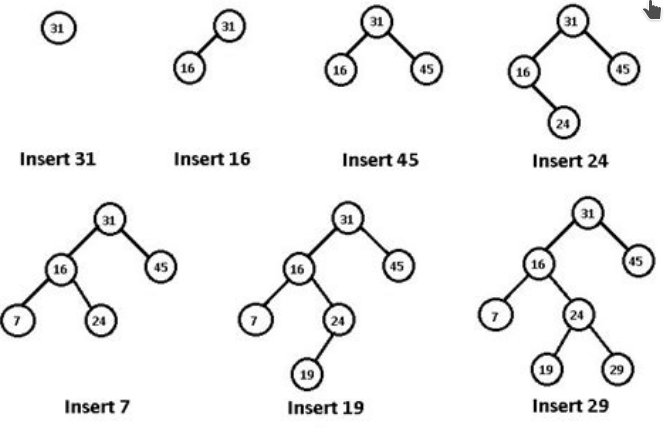
\includegraphics[width=10cm]{bstree.png}
\end{center}

\section*{Prueba unitaria para \emph{Insert} (40\%)}
Crear una pureba unitaria para el metodo \emph{Insert} y colocarla en el proyecto
``BinaryTreeTests''. Este debe verificar que \emph{Insert} funciona correctamente
con un conjunto de numeros de su elecci\'on. \emph{Pista:} Puede utilizar el m\'etodo
\emph{ToArray} para verificar que el m\'etodo funciona correctamente ya que el
arreglo retornado por \emph{ToArray} debe estar ordenado. En otras palabras, el valor
en el indice $i$ debe ser menor o igual al valor en $i+1$.

\end{document}